\chapter{روش پیشنهادی}
در این مقاله برای حل مسئله پیدا کردن استراتژی تخلیه بهینه یک سیستم رایانش لبه‌ای مطابق با شکل \ref{fig-offloading-system} در نظر می‌گیریم.
\begin{figure}[H]
	\centering
	\includegraphics*[width=\textwidth]{figures/MEC5.png}
	\caption{ساختار کلی سیستم تخلیه پردازش}
	\label{fig-offloading-system}
\end{figure}
\newpage
همانطور که در شکل \ref{fig-offloading-system} مشاهده می‌شود، در سامانه مد نظر سه مولفه اصلی زیر وجود دارد:
\begin{enumerate}
	\item دستگاه کاربر (\lr{User Equipment})
	\item سرور پردازش لبه‌ای چند-دسترسی (\lr{Multi-access Edge Computing Server})
	\item کانال بیسیم
\end{enumerate}
در فصل جاری ابتدا نحوه مدل‌سازی هر کدام از این مولفه‌ها شرح داده می‌شود و در انتها الگوریتم و ساختار نرم‌افزاری جدیدی ارائه می‌شود که می‌توان با استفاده از آن استراتژی تخلیه بهینه را به ازای یک سیستم داده شده محاسبه کرد.
\section{مدل وظایف}
فرض می‌شود که \(k\) نوع وظیفه مختلف در سیستم رایانش لبه‌ای وجود دارد و به ازای هر نوع وظیفه دقیقا یک صف در سیستم موجود است. وظایف نوع \(i\)-اُم برای اجرا به صورت محلی\LTRfootnote{Local} احتیاج به \(L_i\) بازه زمانی پردازش توسط واحد پردازنده دارند و به منظور تخلیه به سرور رایانش لبه‌ای احتیاج به \(M_i\) واحد زمانی ارسال توسط واحد ارسال\LTRfootnote{Transmission Unit} دارند. علاوه بر این فرض می‌شود که وظایف نوع \(i\)-اُم در سرور رایانش لبه‌ای به \(C_i\) بازه زمانی پردازش توسط سرور دارند. در ادامه این مقاله برای اشاره به یک واحد زمانی اجرا توسط پردازنده از عبارت \textbf{«قسمت»}\LTRfootnote{Section} استفاده می‌کنیم که انتزاعی از قسمت‌های کد اجرایی است. و برای اشاره به یک واحد زمانی ارسال توسط واحد ارسال از عبارت\textbf{ «بسته» }استفاده می‌شود.
\newpage
\section{مدل دستگاه کاربر}
\label{sec:ue-model}
دستگاه کاربر مطابق با شکل \ref{fig-offloading-system} شامل دو مولفه پردازنده و واحد ارسال می‌باشد. همچنین همانطور که اشاره شد \(k\) صف مختلف به ازای هر کدام از انواع وظایف در سیستم وجود دارد. ظرفیت هر صف را برابر با مقدار ثابت \(Q\) در نظر می‌گیریم. \\

در هر بازه زمانی، واحد پردازنده یا به اندازه یک قسمت پردازش انجام می‌دهد و یا بیکار\LTRfootnote{Idle} است. اجرای هر قسمت پردازش توسط پردازنده به میزان \(P_loc\) توان مصرف می‌کند. به طور مشابه واحد ارسال در هر بازه زمانی یا یک بسته را به شبکه ارسال می‌کند یا بیکار است. نکته قابل توجه در مورد واحد ارسال این است که با توجه به شرایط کانال بیسیم، در یک بازه زمانی خاص ممکن است ارسال موفقیت آمیز باشد یا نباشد. فرض می‌شود که ارسال موفقیت آمیز هر بسته به میزان \(P_tx\) توان مصرف می‌کند. توضیحات بیشتر در مورد نحوه کارکرد کانال بی‌سیم در بخش \ref{sec:wireless} آورده شده است. \\

با توجه به توضیحات داده شده می‌توان مدلی برای «حالت دستگاه کاربر»\LTRfootnote{User Equipment State} تعریف کرد. در مقاله \cite{Liu} برای مشخص کردن حالت دستگاه در زمان \(t\) از یک سه تایی مانند $\boldsymbol{\tau}[t]=\left(q[t], c_{T}[t], c_{L}[t]\right)$ استفاده شده است، که در آن \(q[t]\) مشخص کننده تعداد وظایف موجود در صف وظایف، \(c_T[t]\) مشخص کننده اندیس بسته ارسالی توسط واحد ارسال، و \(c_L[t]\) مشخص کننده اندیس قسمت\LTRfootnote{Section} اجرایی توسط پردازنده است. همچنین حالت \(c_T[t] = 0\) را معادل با بیکار بودن واحد ارسال و \(c_L[t] = 0\) را معادل بیکار بودن واحد پردازنده تعریف می‌کنیم. به عنوان نمونه سه تایی \((4, 2, 1)\) به این معنی است که ۴ وظیفه در صف وظایف وجود دارد، واحد پردازش در حال تخلیه وظیفه‌ای است و تا کنون یک بسته از آن وظیفه را ارسال کرده و به عنوان قدم بعدی باید بسته شماره ۲ را ارسال کند. واحد پردازنده نیز در حال اجرای وظیفه‌ای به صورت محلی است و تا کنون یک قسمت از آن وظیفه را اجرا کرده است. \\
\newpage
با این حال مدل فوق برای مسئله تخلیه وظایف ناهمگون قابل استفاده نیست و نیاز به تغییر دارد. ما در این مقاله برای تعیین حالت دستگاه کاربر از یک چندتایی\LTRfootnote{Tuple} به طول \(k + 4\) مطابق با رابطه \ref{eg:state} استفاده می‌کنیم. در این رابطه متغیرهای \(q_1[t]\) تا \(q_k[t]\) تعداد وظایف موجود از هر یک انواع وظیفه را در صف مربوطه مشخص می‌کنند. متغیرهای \(c_R[t]\) و \(c_L[t]\) مشابه مقاله \cite{Liu} تعریف می‌شوند و به ترتیب وضعیت واحد ارسال و واحد پردازنده را مشخص می‌کنند. دو متغیر جدید \(T_R[t]\) و \(T_L[t]\) به ترتیب مشخص کننده نوع وظیفه در حال ارسال توسط واحد ارسال و نوع وظیفه در حال اجرا توسط پردازنده اند.

\begin{equation}
	\label{eg:state}
	\tau[t]=\left(q_{1}[t], q_{2}[t], \ldots, q_{k}[t], c_{R}[t], c_{L}[t], T_{R}[t], T_{L}[t]\right)
	\forall 0 \leq i \leq k q_{i}[t] \in\{0,1, \cdots, Q\}
\end{equation}
رابطه \ref{eq:state-space} شروط حاکم بر متغیرهای فضای حالت مسئله را عنوان می‌کند و به عبارتی توصیف‌گر فضای حالت مسئله است. در این رابطه عبارت \(\tau(X)\) مقدار متغیر \(X\) در حالت \(\tau\) را مشخص می‌کند.

\begin{equation}
	\label{eq:state-space}
	\begin{aligned}
		&\forall \tau \in S, i \in \{1,2, \ldots, k\} \quad 0 \leqslant\tau\left(q_{i}[t]\right) \leqslant Q\\
		&\forall \tau \in S \quad  \tau\left(T_L[t]\right),  \tau\left(T_R[t]\right) \in \{0, 1,2, \ldots, k\}\\
		&\left.\forall \tau \in\left\{\tau^{\prime} \in S \mid \tau^{\prime}\left(T_{R}\right)=0\right\} \quad \tau(C_R[t]\right)=0\\
		&\forall \tau \in\left\{\tau^{\prime} \in S \mid \tau^{\prime}\left(T_{R}\right) \neq 0\right\} \quad 1 \leqslant \tau\left(C_{R}[t]\right) \leqslant M_{T_{R}[t]} \\
		&\left.\forall \tau \in\left\{\tau^{\prime} \in S \mid \tau^{\prime}\left(T_{L}\right)=0\right\} \quad \tau(C_L[t]\right)=0\\
		&\forall \tau \in\left\{\tau^{\prime} \in S \mid \tau^{\prime}\left(T_{L}\right) \neq 0\right\} \quad 1 \leqslant \tau\left(C_{L}[t]\right) \leqslant L_{T_{R}[t]} - 1
	\end{aligned}
\end{equation}

\newpage
\section{مدل زمان}
در مدل مسئله وضعیت سیستم در فواصل زمانی\LTRfootnote{Time Slot} با طول ثابت \(\Delta\) میلی ثانیه بررسی می‌شود. برای مثال حالت دستگاه کاربر را در بازه زمانی \(t\)-اُم با \(\tau[t]\) مشخص می‌کنیم، و حالت دستگاه در بازه زمانی \(t + 1\) را با \(\tau[t + 1]\) مشخص می‌کنیم و فاصله بین این دو بازه زمانی \(\Delta\) میلی ثانیه است. \\

بررسی زمان به صورت واحدهای گسسته به منظور ساده‌سازی مسئله و همچنین گسترش پذیری آن به شرایط محیطی مختلف صورت گرفته است. در عمل، یک مقدار قابل استفاده برای \(\Delta\) طول بازه‌های زمانی شبکه دسترسی\LTRfootnote{Access Network} مورد نظر است. برای مثال در شبکه‌های \lr{LTE} طول هر بازه زمانی ۰/۵ میلی‌ثانیه می‌باشد. \cite{LTE}

\section{مدل کانال بیسیم}
\label{sec:wireless}
در این مقاله مشابه با \cite{Liu} کانال بی‌سیم را به صورت تصادفی مدل می‌کنیم\LTRfootnote{Stochastic Channel} زیرا با توجه به ناپایداری کانال در ارتباطات بیسیم، به خصوص در شبکه‌های تلفن همراه، ارسال بسته‌ها توسط واحد ارسال لزوما موفقیت آمیز نخواهد بود. برای کانال بی‌سیم یک مدل ساده احتمالی به این صورت در نظر می‌گیریم که که ارسال هر بسته با احتمال \(\beta\) موفقیت آمیز خواهد بود و با احتمال \(1 - \beta\) ناموفق خواهد بود. در عمل مقدار \(\beta\) با توجه به رابطه \ref{eq:shannon} (رابطه شنون) محاسبه می‌شود، که در آن \(R\) مشخص کننده سایز هر بسته است، \(B\) پهنای باند سیستم، \(\gamma[t]\) مقدار بهره کانال\LTRfootnote{Channel Gain} و \(N_0\) مشخص کننده اندازه نویز کانال است.
\begin{equation}
	\label{eq:shannon}
		\begin{aligned}
				&\beta=P(r(t) \geq R) \\
				&r(t)=B \log _{r}\left(1+\frac{\gamma[t] P_{\mathrm{tx}}}{N_0 B}\right)
		\end{aligned}
\end{equation}
\section{مفهوم کنش}
یک استراتژی تخلیه در هر بازه زمانی مانند \(t\) می‌بایست یک کنش\LTRfootnote{Action} مانند \(A[t]\) را برای اجرا توسط دستگاه کاربر انتخاب کند. برای درک مفهوم کنش، ابتدا مشابه \cite{Liu} حالتی را در نظر می‌گیریم که تنها یک صف (یعنی یک نوع وظیفه) در سیستم وجود داشته باشد. در این حالت می‌توانیم مجموعه کنش‌ها را با چهار عضو مطابق جدول \ref{table:actions} مشخص کنیم.

\begin{table}[H]
	\centering
	\begin{latin}
			\begin{tabular}{@{}lrll@{}}
			\toprule
			\textbf{ID} & \textbf{Transmit} & \textbf{Local Execution} & \textbf{Description} \\ \midrule
			1           & False             & False                    & No operation         \\
			2           & False             & True                     & Add to CPU           \\
			3           & True              & False                    & Add to TU            \\
			4           & True              & True                     & Add to both units    \\ \bottomrule
		\end{tabular}
	\end{latin}
	\caption{لیست کنش‌ها در سیستم با یک صف وظیفه}
	\label{table:actions}
\end{table}
در حالتی که بیش از یک صف در سیستم وجود دارد به نحو مشابه می‌توان تعداد کنش‌های ممکن را مطابق با جدول \ref{table:actions-multiqueue} بدست آورد.
\begin{table}[H]
	\begin{latin}
		\begin{tabular}{@{}lrlll@{}}
			\toprule
			\textbf{ID}                     & \textbf{Transmit} & \textbf{Local Execution} & \textbf{Description} & \textbf{Count}                \\ \midrule
			$\{1\}$                           & False             & False                    & No operation         & 1                    \\
			$\{2, ..., k + 1\}$               & False             & True                     & Add to CPU           & $k$                    \\
			$\{k + 2, ..., 2k + 1\}$          & True              & False                    & Add to TU            & $k$                    \\
			$\{2k + 2, ..., 2k + k * k - 1\}$ & True              & True                     & Add to both units    & $k^2$ \\ \bottomrule
		\end{tabular}
	\end{latin}
	\caption{دسته‌بندی کنش‌ها در سیستم با $k$ صف}
	\label{table:actions-multiqueue}
\end{table}
اجرای هر کنش طبعا ممکن است که حالت سیستم را تغییر دهد. به طور مثال اجرای هر عمل نوع ردیف دوم یک وظیفه را از صف مربوطه برداشته بنابراین طول صف به شکل (\(q_i[t + 1] = q_i[t] - 1\) تغییر می‌کند، همچنین وضعیت پردازنده را از \(c_L[t] = 0\) یعنی حالت بیکار به \(c_L[t + 1] = 1\) تغییر خواهد کرد زیرا قسمت اول وظیفه مربوطه در بازه زمانی \(t\) حتما انجام می‌شود. به طور مشابه برای سایر کنش‌ها نیز میتوان توابع انتقال\LTRfootnote{Transition Function} مشخص تعریف کرد که با گرفتن یک حالت ورودی، حالت خروجی را محاسبه نماید. به دلیل پیچیدگی و حجم زیاد معادلات این توابع از توضیح بیشتر در این بخش صرف نظر شده است. برای مشاهده منطق دقیق این توابع در قالب کد، به پیوست ۱ مراجعه شود.

\section{روند فعالیت سیستم تخلیه وظایف}
دستگاه کاربر در هر سیکل زمانی به ترتیب مشخص شده در شکل \ref{fig:ueproc} فعالیت می‌کند.
\begin{figure}[H]
	\centering
	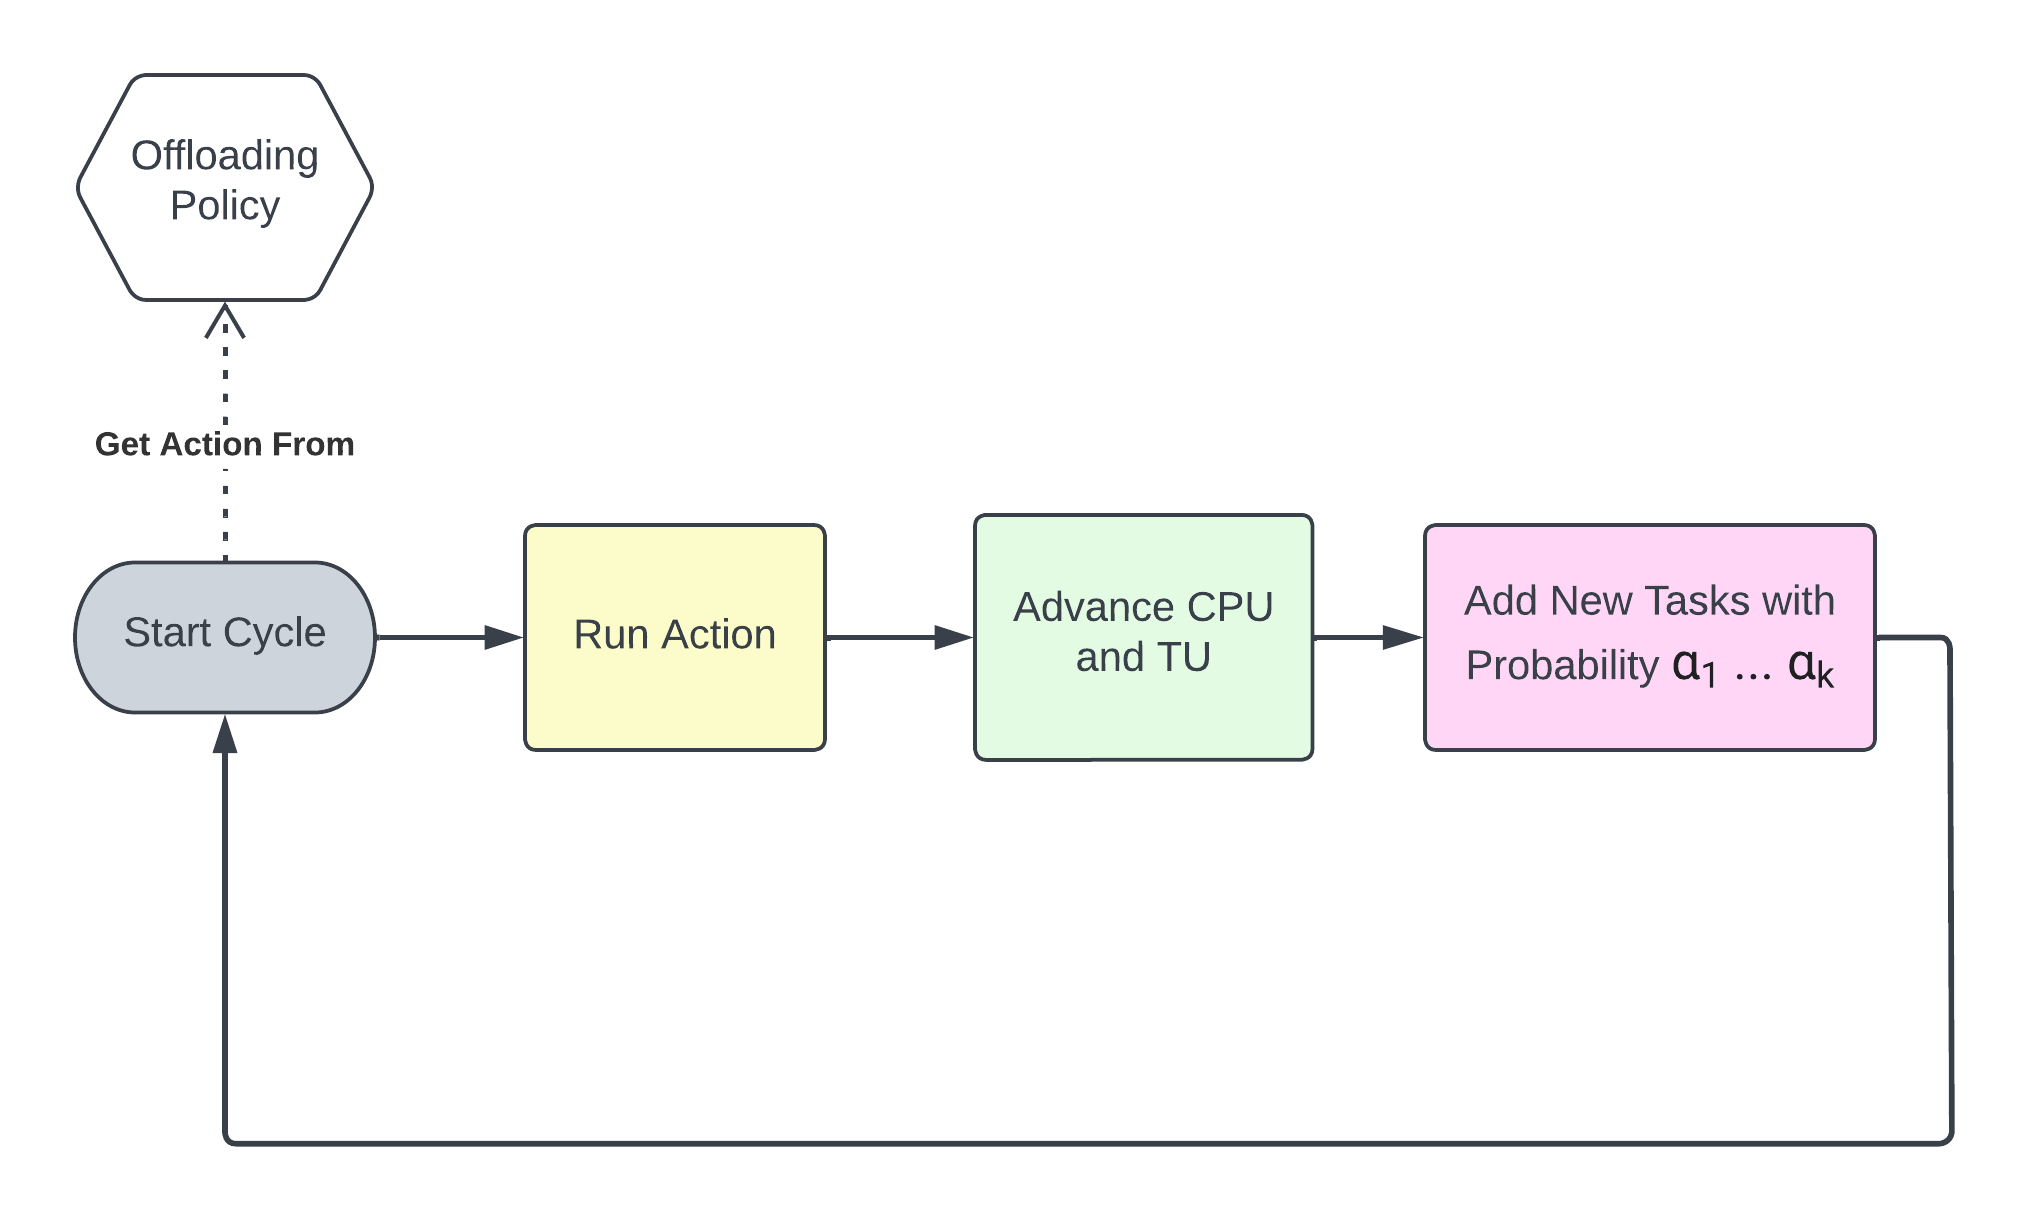
\includegraphics[width=\textwidth]{figures/ueproc.png}
	\caption{روند فعالیت دستگاه کاربر}
	\label{fig:ueproc}
\end{figure}

\section{استراتژی تخلیه تصادفی}
با استفاده از مدل‌های توصیف شده در بخش‌های قبل، حال می‌توانیم یک تعریف ریاضی از «استراتژی تخلیه تصادفی» داشته باشیم. مشابه با مقاله \cite{Liu} یک استراتژی تخلیه تصادفی را به صورت توزیع احتمالی مانند \(g_\tau^a\) بر روی مجموعه \(S \times A\) تعریف می‌کنیم. در اینجا عبارت \(S \times A\) نمایانگر ضرب دکارتی مجموعه تمام حالت‌های سیستم در مجموعه تمام کنش‌های ممکن در سیستم است. یک نکته قابل توجه این است که برخی از دو تایی‌های حاصل از این ضرب دکارتی هیچ گاه در واقعیت امکان‌پذیر نیست. برای مثال در حالتی که صف خالی باشد تنها یک کنش امکان پذیر است و آن هم کنش شماره ۱ (\lr{No Operation}) است. با این حال برای سادگی در توضیح تئوری روش حل مسئله، این دو تایی‌ها را نیز در دامنه تابع توزیع احتمالی استراتژی تخلیه در نظر می‌گیریم تا همواره اندازه دامنه تابع احتمال برابر با مقدار ثابت \(|S| \cdot |A|\) باشد اما در پیاده‌سازی عملی چنین دوتایی‌هایی از دامنه حذف می‌شوند و مقدار احتمال ثابتی برابر صفر می‌گیرند تا با کاهش فضای حالت مسئله، سرعت الگوریتم اجرایی بهبود یابد. \\

همچنین طبق تعریف توزیع احتمال، رابطه \ref{eq:prob} باید برای هر استراتژی تخلیه تصادفی برقرار باشد.
\begin{equation}
	\label{eq:prob}
	\sum_{\tau \in S} \sum_{a \in A} g_{\tau}^{a}=1
\end{equation}
\newpage
\section{مدل زنجیره مارکوف دستگاه کاربر}
به منظور محاسبه معیارهایی مانند توان مصرفی میانگین و تاخیر سرویس میانگین لازم است که بتوانیم درباره وضعیت سیستم تخلیه وظیفه در طولانی‌مدت استنتاج کنیم. در این قسمت ابتدا مدل آماری زنجیره مارکوف گسسته-زمان را معرفی می‌کنیم و سپس توضیح می‌دهیم که چگونه می‌توان با استفاده از این مدل معیارهای تاخیر و توان میانگین را برای یک سیستم تخلیه وظیفه محاسبه کرد.
\begin{defi}
\label{def:one}
دنباله‌ای از متغیرهای تصادفی $X_{1}, X_{2}, \ldots$ را که احتمال تغییر وضعیت از زمان $t$ به $t + 1$ مستقل از وضعیت‌های قبلی باشد را یک \textbf{زنجیره مارکوف گسسته-زمان} می‌نامند. این گزاره را به بیان متغیرهای تصادفی و تابع احتمال به صورت رابطه زیر نشان می‌دهیم.
\begin{equation*}
	\operatorname{Pr}\left(X_{t+1}=x \mid X_{1}=x_{1}, X_{2}=x_{2}, \ldots, X_{n}=x_{t}\right)=\operatorname{Pr}\left(X_{t+1}=x \mid X_{t}=x_{t}\right)
\end{equation*}
\end{defi}
\begin{defi}
\label{def:two}
زنجیره مارکوف گسسته زمان $X(t)$ را \textit{همگن-زمان} می‌گوییم اگر شرط زیر همواره برقرار باشد:
\begin{equation*}
P\left(X_{n+1}=j \mid X_{n}=i\right)=P\left(X_{1}=j \mid X_{0}=i\right)
\end{equation*}
به عبارت دیگر یعنی احتمالات مربوط به انتقال بین حالت‌ها به زمان \(t\) وابسته نیستند. در این حالت احتمال انتقال زنجیره از حالت \(i\) به \(j\) را با عبارت $p_{i j}=P\left(X_{1}=j \mid X_{0}=i\right)$ نمایش می‌دهیم و همچنین ماتریس انتقال را با $P=\left(p_{i j}\right)$ نمایش می‌دهیم.
\end{defi}
طبق تعاریف \ref{def:one} و \ref{def:two} وضعیت دستگاه کاربر در سیستم تخلیه وظیفه را می‌توان به یک زنجیره مارکوف گسسته-زمان همگن-زمان تشبیه کرد که در آن حالت دستگاه کاربر در زمان $t$ را با $\tau[t]$ نشان می‌دهیم و همچنین ماتریس انتقال $\chi$ را برای زنجیره در نظر می‌گیریم به طوری که $\chi_{\tau, \tau^{\prime}}$ احتمال انتقال از حالت $\tau$ به \(\tau^{\prime}\) را مشخص می‌کند.

\clearpage